% =============================================================================
%  HyperSpatial — HPC extended abstract (IEEE conference format, 2 pages)
%  Compile:  tectonic hpc_abstract.tex      (or: pdflatex hpc_abstract.tex twice)
%  Every number below was measured on the EnMAP test scene; raw data in
%  benchmarks/results/engine_benchmark.csv and engine_tile_sweep.csv.
% =============================================================================
\documentclass[conference]{IEEEtran}
\IEEEoverridecommandlockouts
\usepackage{amsmath}
\usepackage{booktabs}
\usepackage{multirow}
\usepackage[table]{xcolor}
\usepackage{pgfplots}
\pgfplotsset{compat=1.18}
\usepackage[hidelinks]{hyperref}

\definecolor{hsblue}{HTML}{2A78D6}
\definecolor{hsorange}{HTML}{EB6834}
\definecolor{hsgreen}{HTML}{1BAF7A}
\definecolor{hsamber}{HTML}{EDA100}
\definecolor{hsgrey}{HTML}{8A8984}

\begin{document}

\title{Out-of-Core, Tile-Parallel Hyperspectral Processing on Commodity
Hardware: an OpenMP/OpenCL Engine Integrated with QGIS}

\author{\IEEEauthorblockN{Aaron R}
\IEEEauthorblockA{\textit{Digital University Kerala}\\
Thiruvananthapuram, Kerala, India\\
aaronr43210@gmail.com}}

\maketitle

% ------------------------------------------------------------------ abstract
\begin{abstract}
Spaceborne imaging spectrometers such as EnMAP deliver scenes of hundreds of
spectral bands; a single 224-band EnMAP L2A scene used here is 686\,MB and
holds about $2.4\times10^{8}$ reflectance values. Desktop GIS tools typically
process such cubes in memory, which limits them on laptops. We present
\texttt{hyperspatial\_cli}, a C++17 engine that decomposes a scene into
independent tiles and processes them out of core: OpenMP threads with
dynamic scheduling and thread-private GDAL handles compute seven spectral
indices, a two-pass principal component analysis and the Spectral Angle
Mapper, and a portable OpenCL~1.2 backend runs the same kernels on GPUs of any
vendor with a per-tile CPU fallback. The engine is driven from QGIS by a
binary-free plugin that never blocks the user interface, and its GeoTIFF tiles
are the unit of distribution for downstream Apache Spark analytics. On a
12-core Apple M4 Pro all seven indices of the whole scene take 2.02\,s
(256-px tiles, 8 threads), SAM 0.99\,s and PCA 5.96\,s, with peak memory set
by threads and tile size rather than scene size. A tile-size sweep shows that
granularity limits scaling: the 8-thread speed-up rises from $1.2\times$ with
4 tiles to $5.7\times$ with 100 tiles, until per-tile overhead dominates.
CPU and GPU outputs agree to float rounding, except one pixel in
$1.5\times10^{6}$ for two indices. The GPU backend is not faster on this
machine: the workload is I/O-bound and the driver forces a single host
thread in GPU mode. We report these measurements and the design lessons they
imply.
\end{abstract}

\begin{IEEEkeywords}
hyperspectral imaging, OpenMP, OpenCL, out-of-core processing,
heterogeneous computing, GIS, EnMAP
\end{IEEEkeywords}

% ------------------------------------------------------------------ I
\section{Introduction}
Imaging spectroscopy missions (EnMAP~\cite{guanter2015enmap}, PRISMA, EMIT) produce cubes whose size
grows with the number of bands rather than only with area. Most users of
these data work in desktop GIS, where open-source hyperspectral tools commonly
hold the cube in memory, and GPU acceleration is mainly found in commercial or
NVIDIA-specific software~\cite{qu2013sam}. Portable OpenCL implementations of
hyperspectral kernels have been studied as research
prototypes~\cite{bernabe2019opencl}; our focus is an engineering one: making
full-scene processing fast, memory-bounded and robust on the hardware GIS users
already own, inside the GIS. Contributions:
(i) an out-of-core, tile-parallel engine with a closed-form memory model;
(ii) a vendor-portable OpenCL backend with per-tile CPU fallback;
(iii) a measured evaluation on a real EnMAP scene, including a negative GPU
result and its cause.

% ------------------------------------------------------------------ II
\section{Engine Design}
\subsection{Decomposition and out-of-core streaming}
A tiler splits the $W\times H\times B$ scene ($1259\times1216\times224$) into
square tiles of side $s$ (default 512\,px, 9 tiles). For the index pipeline
tiles are independent, so the problem is embarrassingly parallel. Each worker
reads one tile, runs a six-stage pipeline (read, no-data handling, bad-band
masking, indices, per-band normalisation, write) and writes one GeoTIFF with
$B+7$ bands. The scene is never resident; with $T$ threads the working set is
\begin{equation}
M \approx T\, s^{2} B \cdot 4\ \text{bytes} \;(\approx T\times 235\,\text{MB at } s=512),
\end{equation}
independent of scene size.

\subsection{Shared-memory parallelism}
The tile loop is an OpenMP \texttt{parallel for} with \texttt{schedule(dynamic)},
because edge tiles of a rotated satellite footprint carry far less work
(up to 97\,\% background). GDAL datasets are not thread-safe, so every read
opens a thread-private handle and every tile is written to its own file; the
only shared state is the first error, guarded by an atomic flag and a mutex.
No exception may leave the parallel region: each iteration catches, records
and continues, and the process exits with code~2.

\subsection{Heterogeneous backend}
The OpenCL~1.2 backend selects a GPU device on Apple, NVIDIA, Intel or AMD
platforms. Its index kernel is a line-for-line port of the CPU code;
SAM~\cite{kruse1993sips} and PCA have dedicated kernels, the latter with Kahan-compensated
float32 reductions. Any initialisation or dispatch failure falls back to the
CPU for that tile. Because the Apple OpenCL queue was observed to corrupt
results when fed from several host threads, GPU mode runs the tile loop on a
single host thread.

\subsection{Numerical robustness and integration}
PCA uses two passes in double precision (exact means, then
$\Sigma(x-\mu)(x-\mu)^{T}$), a Jacobi eigensolver with a deterministic sign
convention, and a projection pass. Bands are selected by wavelength from file
metadata. A QGIS plugin launches the engine as a subprocess from a worker
thread, streams its progress and loads styled layers; the tiles feed Apache
Sedona jobs on Spark unchanged, complementing cluster-scale Spark
processing of hyperspectral data~\cite{wu2016spark}.

% ------------------------------------------------------------------ III
\section{Evaluation}
\textbf{Setup.} EnMAP L2A scene (Tyrolean Alps, 12 June 2022); Apple M4 Pro
(8 performance + 4 efficiency cores, 24\,GB); engine time from its
\texttt{RESULT} line, median of three runs.

\begin{figure}[t]
\centering
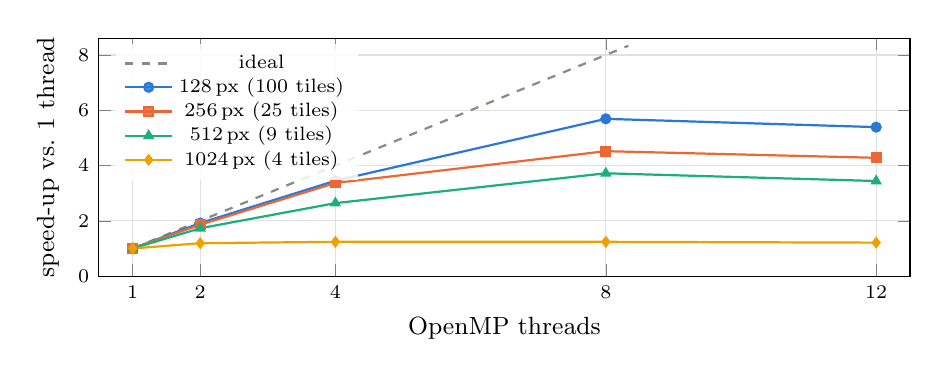
\begin{tikzpicture}
\begin{axis}[
  width=0.98\columnwidth, height=4.6cm,
  xlabel={OpenMP threads}, ylabel={speed-up vs.\ 1 thread},
  xmin=0.5, xmax=12.5, ymin=0, ymax=8.6, restrict y to domain=0:8.6,
  xtick={1,2,4,8,12}, ytick={0,2,4,6,8},
  grid=major, grid style={hsgrey!25},
  legend style={font=\scriptsize, at={(0.02,0.98)}, anchor=north west, draw=none, fill=white, fill opacity=0.85, text opacity=1, row sep=-2pt},
  tick label style={font=\scriptsize}, label style={font=\small},
  every axis plot/.append style={thick, mark size=1.6pt}]
\addplot[hsgrey, dashed, mark=none, domain=1:12] {x};
\addlegendentry{ideal}
\addplot[hsblue, mark=*] coordinates {(1,1.00) (2,1.92) (4,3.45) (8,5.69) (12,5.39)};
\addlegendentry{128\,px (100 tiles)}
\addplot[hsorange, mark=square*] coordinates {(1,1.00) (2,1.86) (4,3.37) (8,4.52) (12,4.28)};
\addlegendentry{256\,px (25 tiles)}
\addplot[hsgreen, mark=triangle*] coordinates {(1,1.00) (2,1.73) (4,2.64) (8,3.72) (12,3.44)};
\addlegendentry{512\,px (9 tiles)}
\addplot[hsamber, mark=diamond*] coordinates {(1,1.00) (2,1.19) (4,1.24) (8,1.24) (12,1.21)};
\addlegendentry{1024\,px (4 tiles)}
\end{axis}
\end{tikzpicture}
\caption{Strong scaling of the seven-index pipeline on the whole scene for
several tile sizes. Smaller tiles expose more parallelism.}
\label{fig:scaling}
\end{figure}

\begin{table}[t]
\centering
\caption{Whole-scene runtime, memory and CPU--GPU agreement}
\label{tab:ops}
\setlength{\tabcolsep}{4pt}
\begin{tabular}{@{}lrrrl@{}}
\toprule
Operation & 1 thr. & best CPU & GPU & max $|\text{CPU}-\text{GPU}|$ \\
\midrule
Indices (7)   & 8.60\,s & 2.52\,s & 9.13\,s & $\le\!1.5{\times}10^{-5}$\,$^{a}$ \\
SAM           & ---     & 0.99\,s & 1.15\,s & $1.1{\times}10^{-6}$\,rad \\
PCA (3 PCs)   & ---     & 5.96\,s & 5.79\,s & $1.6{\times}10^{-5}$ of range \\
\midrule
Peak memory   & 1.38\,GB & 4.21\,GB & 1.39\,GB & \\
\bottomrule
\end{tabular}\\[2pt]
{\scriptsize $^{a}$\,Except one pixel in $1.5\times10^{6}$ for NDVI and NDWI
(zero-operand edge case). 512-px tiles; best CPU: 8 threads (indices),
12 threads (SAM, PCA); from \texttt{engine\_benchmark.csv}. Fig.~\ref{fig:scaling}
uses a separate sweep (\texttt{engine\_tile\_sweep.csv}); single-thread times
differ by up to 9\,\% between the two sessions.}
\end{table}

\textbf{Scaling.} Fig.~\ref{fig:scaling} shows that tile granularity, not
core count, limits scaling. With the default 512-px tiles the scene has only 9
tiles, which cannot be balanced over 8 threads (one thread processes two), so
8 threads give $3.7\times$ (46\,\% efficiency). Finer tiles expose more
parallelism: $4.5\times$ with 256-px tiles (25 tiles) and $5.7\times$ with
128-px tiles (100 tiles), whereas 1024-px tiles (4 tiles) saturate at
$1.2\times$. Finer tiles also add per-tile overhead (one thread needs 20.5\,s at
128\,px against 9.1\,s at 256\,px), so the fastest configuration is 256-px
tiles on 8 threads: \textbf{2.02\,s} for all seven indices, 20\,\% faster than
the 512-px default and with 2.73 instead of 4.15\,GB peak memory. No
configuration improves beyond 8 threads; we attribute this to the four
efficiency cores and to I/O (reading 686\,MB, LZW-compressing 1\,GB), to be
confirmed by an instrumented read/compute/write breakdown.

\textbf{Memory.} Peak resident memory grows with threads (1.38\,GB serial,
2.46\,GB with 2, 4.21\,GB with 8 threads) and stays bounded because at most
one tile per thread is in flight, matching Eq.~(1).

\textbf{CPU vs.\ GPU.} Table~\ref{tab:ops}: the GPU path reproduces the CPU
results but is not faster. Indices perform a few operations per value, so
time is dominated by reading the 686\,MB cube and compressing 1\,GB of output;
in GPU mode that I/O runs on one host thread, and the GPU run (9.13\,s)
matches the serial CPU run (8.53\,s). For SAM and PCA the GPU is on par with
12 CPU threads, while SAM's GPU run needs 0.67\,GB instead of 2.53\,GB.

% ------------------------------------------------------------------ IV
\section{Conclusion and Future Work}
A tile-parallel, out-of-core design processes a complete 224-band scene in
seconds on a laptop with bounded memory, and a portable OpenCL backend
reproduces the CPU results on a non-NVIDIA GPU. The measurements point to the
next steps: a 256-px default tile size, a pipelined hybrid mode (multithreaded tile I/O feeding one GPU
dispatch thread), evaluation on x86 servers with discrete GPUs, weak scaling
over multi-scene mosaics, and distribution of tiles across a Spark cluster.

% ------------------------------------------------------------------ refs
\begin{thebibliography}{9}
\bibitem{guanter2015enmap} L.~Guanter \emph{et al.}, ``The EnMAP spaceborne
imaging spectroscopy mission for Earth observation,'' \emph{Remote Sensing},
vol.~7, no.~7, pp.~8830--8857, 2015, doi:10.3390/rs70708830.
\bibitem{qu2013sam} H.~Qu, J.~Zhang, Z.~Lin, and H.~Chen, ``Parallel
acceleration of SAM algorithm and performance analysis,'' \emph{IEEE J. Sel.
Topics Appl. Earth Observ. Remote Sens.}, vol.~6, no.~3, pp.~1172--1178, 2013,
doi:10.1109/JSTARS.2013.2239261.
\bibitem{bernabe2019opencl} S.~Bernab\'e \emph{et al.}, ``Portability study of
an OpenCL algorithm for automatic target detection in hyperspectral images,''
\emph{IEEE Trans. Geosci. Remote Sens.}, vol.~57, no.~11, pp.~9499--9511, 2019,
doi:10.1109/TGRS.2019.2927077.
\bibitem{kruse1993sips} F.~A.~Kruse \emph{et al.}, ``The spectral image
processing system (SIPS) --- interactive visualization and analysis of imaging
spectrometer data,'' \emph{Remote Sens. Environ.}, vol.~44, no.~2--3, pp.~145--163,
1993, doi:10.1016/0034-4257(93)90013-N.
\bibitem{wu2016spark} Z.~Wu, Y.~Li, A.~Plaza, J.~Li \emph{et al.}, ``Parallel
and distributed dimensionality reduction of hyperspectral data on cloud
computing architectures,'' \emph{IEEE J. Sel. Topics Appl. Earth Observ. Remote
Sens.}, vol.~9, no.~6, pp.~2270--2278, 2016, doi:10.1109/JSTARS.2016.2542193.
\end{thebibliography}

\end{document}
